\documentclass[12pt,a4paper]{article}
\usepackage[margin=20mm]{geometry}
\usepackage{fontspec}
\setmainfont{Arial}
\setmonofont{Menlo}[Scale=0.85]
\usepackage[russian]{babel}
\usepackage{booktabs,longtable,array}
\usepackage{xcolor}
\usepackage{graphicx}
\usepackage{fancyvrb}
\usepackage{hyperref}
\hypersetup{colorlinks=true,urlcolor=blue,linkcolor=black}
\setlength{\parindent}{0pt}
\setlength{\parskip}{5pt}
\setlength{\emergencystretch}{3em}
\DefineVerbatimEnvironment{Code}{Verbatim}{fontsize=\small,frame=single,framesep=3mm}
\title{Лабораторная работа № 2\\[4mm]\large Настройка SCR1 и обработка исключений\\Вариант 9}
\author{}
\date{}
\begin{document}
\maketitle

\section{Цель и параметры задания}
Изучить настройку архитектуры системы команд SCR1, механизм исключений и
согласование аппаратных адресов входа с размещением программы компоновщиком.

\begin{center}
\begin{tabular}{ll}
\toprule
Параметр & Вариант 9 \\
\midrule
Исключение & Illegal instruction --- недопустимая инструкция \\
Тест & \texttt{isa/rv32mi/illegal.S} \\
Reset Vector & \texttt{0xF00} \\
Trap Vector & \texttt{0xB00} \\
Сообщение обработчика & \texttt{incorrect instruction} \\
Рабочая ветка & \texttt{lab\_scr1\_sim} \\
\bottomrule
\end{tabular}
\end{center}

\section{Окружение и подготовка репозитория}
Использовано Docker-окружение на базе Ubuntu 24.04 с RISC-V GCC и
Verilator 5.030. Симулятор собран из исходников согласно Dockerfile.
Симуляция выполнялась в контейнере, исходники доступны в
\texttt{/work/scr1}. Для ядра выбраны \texttt{CFG=MAX}, интерфейс
\texttt{BUS=AHB}, архитектура RV32IMC.

Изначально была клонирована копия SCR1; позднее удалённый \texttt{origin}
настроен на личный репозиторий по SSH:
\begin{Code}
git@github.com:ProshkaAnastasia/scr1.git
\end{Code}
Исходный репозиторий Syntacore сохранён как \texttt{upstream}.
Работа выполнена в ветке \texttt{lab\_scr1\_sim}.

\section{Исходная проверка и выбор одного теста}
До изменения обработчика и адресов сохранён базовый прогон ISA-набора:
\begin{Code}
make TARGETS="riscv_isa"
\end{Code}
Все 56 тестов набора \texttt{riscv\_isa} прошли успешно.
Результаты сохранены в \path{report/results/baseline/test_results.txt},
журнал запуска --- в \texttt{baseline.log} в том же каталоге.

Затем файл \path{sim/tests/riscv_isa/rv32_tests.inc} заменён строкой:
\begin{Code}
rv32_isa_tests := isa/rv32mi/illegal.S
\end{Code}
Удалены остальные добавления списка, включая условные блоки расширений M и C.
Параметр \texttt{TARGETS=riscv\_isa} выбирает набор, а этот файл ограничивает
его единственной программой. Отключение тестов M/C не отключает расширения ядра.
Одиночный прогон до изменения обработчика также завершился \texttt{1/1 PASS};
его журнал сохранён в \path{report/results/illegal_before.log}.

\section{Изменения аппаратных параметров и размещения программы}

\subsection{Адреса в RTL}
В \path{src/includes/scr1_arch_description.svh} установлены:
\begin{Code}
SCR1_ARCH_RST_VECTOR = 'hF00;
SCR1_ARCH_MTVEC_BASE = 'hB00;
\end{Code}
Первый параметр определяет адрес начала исполнения после сброса.
Второй задаёт базу \texttt{mtvec} после сброса и фиксированные биты,
если они предусмотрены конфигурацией. Он не размещает машинный код
в памяти: размещение требуется согласовать отдельно.

\subsection{Отдельные секции для обработчика и старта}
В \path{sim/tests/common/riscv_macros.h}, внутри \texttt{RVTEST\_CODE\_BEGIN},
код обработчика и стартовый код разнесены:
\begin{Code}
.section .text.trap, "ax", @progbits
trap_vector:
    # обработчик исключений

.section .text.reset, "ax", @progbits
.globl _start
_start:
    # инициализация перед запуском теста
\end{Code}
Флаги \texttt{ax} обозначают размещаемую в памяти исполняемую секцию.
Текст сообщения находится в \texttt{.rodata}; переключение к нему выполнено
через \texttt{.pushsection}/\texttt{.popsection}.

В \path{sim/tests/common/link.ld} заданы выходные секции:
\begin{Code}
.trap 0xB00 : {
    PROVIDE(__TEXT_START__ = .);
    KEEP(*(.text.trap))
} >RAM

.reset 0xF00 : {
    KEEP(*(.text.reset))
    *(.text.init)
} >RAM
\end{Code}
\texttt{KEEP} сохраняет секции даже при удалении неиспользуемого кода.
Относительные смещения \texttt{.org} для размещения обработчика и старта
убраны. Адреса теперь закрепляет компоновщик непосредственно, поэтому
изменение размера обработчика не сдвигает \texttt{\_start}.
Принудительное отключение relaxation для этого не требуется.
Служебные точки выхода симулятора \texttt{SIM\_EXIT=0xF4} и
\texttt{SIM\_STOP=0xF8} сохранены.

\subsection{Подготовка mtvec программой}
Стартовый код устанавливает адрес обработчика также программно:
\begin{Code}
la t0, trap_vector
csrw mtvec, t0
\end{Code}
Таким образом, аппаратная исходная база и программная запись согласованы
с адресом метки \texttt{trap\_vector=0xB00}. Директива \texttt{ENTRY(\_start)}
в linker script задаёт точку входа ELF, но не заменяет аппаратный Reset Vector.

\section{Модификация обработчика trap\_vector}
При исключении аппаратура записывает причину в \texttt{mcause}, адрес
проблемной инструкции в \texttt{mepc} и переходит по \texttt{mtvec}.
Для недопустимой инструкции код причины равен 2.

В начале \texttt{trap\_vector} добавлена проверка и посимвольный вывод:
\begin{Code}
csrr a4, mcause
li a5, CAUSE_ILLEGAL_INSTRUCTION
bne a4, a5, .Lafter_illegal_print
la a4, .Lillegal_message
li t0, 0xf0000000
.Lprint_illegal:
    lbu a5, 0(a4)
    beqz a5, .Lafter_illegal_print
    sb a5, 0(t0)
    addi a4, a4, 1
    j .Lprint_illegal
.Lafter_illegal_print:
    csrr a4, mcause
\end{Code}
В исходном заголовке каждая продолжающая строка макроса завершается
символом обратной косой черты; здесь приведён раскрытый ассемблерный фрагмент.

\begin{Code}
.Lillegal_message:
    .asciz "incorrect instruction\n"
\end{Code}
\texttt{.asciz} добавляет нулевой байт конца строки. \texttt{lbu} читает
очередной символ, \texttt{sb} отправляет его в порт симулятора
\texttt{0xF0000000}. Этот адрес используется также в \texttt{sc\_print.c}.
Вызов C-функции и настройка стека для печати не требуются.

После вывода \texttt{mcause} читается повторно, поскольку \texttt{a4}
в цикле использовался как указатель. Код \texttt{ecall} не равен 2,
поэтому сообщение при завершении теста повторно не печатается.
Существующие проверки \texttt{ecall}, передача управления
\texttt{mtvec\_handler} и выход через \texttt{sc\_exit} сохранены.
Регистры \texttt{a4}, \texttt{a5}, \texttt{t0} здесь являются рабочими;
для выбранного теста его собственный обработчик заново задаёт используемые
\texttt{t0} и \texttt{t1}. Изменение не является универсальным обработчиком
с сохранением полного контекста для произвольной программы.

\section{Как продолжается тест после исключения}
Файл \path{dependencies/riscv-tests/isa/rv32mi/illegal.S} подключает общий
код из \texttt{../rv64mi/illegal.S}, переопределяя макрос режима на RV32.
Первая проверка выполняет:
\begin{Code}
li TESTNUM, 2
bad2:
    .word 0
    j fail
\end{Code}
Нулевое машинное слово должно вызвать исключение. Переход \texttt{j fail}
поймал бы ошибку, если бы процессор продолжил обычное исполнение.

Общий \texttt{trap\_vector} после сообщения передаёт управление
\texttt{mtvec\_handler}, определённому самим тестом.
Объявление \texttt{.weak mtvec\_handler} лишь делает символ необязательным;
его фактический адрес определяется меткой в программе.
Обработчик теста проверяет \texttt{mcause}, \texttt{mepc} и допустимое
содержимое \texttt{mtval}, после чего для \texttt{bad2} выполняет:
\begin{Code}
addi t0, t0, 8
csrw mepc, t0
mret
\end{Code}
Так пропускаются четыре байта \texttt{.word 0} и четыре байта \texttt{j fail}.
В тесте включена \texttt{.option norvc}, поэтому последующая команда
перехода имеет длину четыре байта.

SCR1 поддерживает только Machine mode. Проверка наличия Supervisor mode
не подтверждает его поддержку, поэтому оставшиеся Supervisor-проверки
пропускаются переходом на \texttt{pass}.
Макрос успеха устанавливает \texttt{a0=0} и выполняет \texttt{ecall}.
Это отдельное исключение с \texttt{mcause=11}; общий обработчик направляет
его на \texttt{\_report}, затем \texttt{sc\_exit}. Операционной системы здесь нет.

\section{Итоговая симуляция и проверка адресов}
Для финальной проверки запущено из корня SCR1 внутри контейнера:
\begin{Code}
make run_verilator CFG=MAX BUS=AHB TARGETS=riscv_isa TRACE=1
\end{Code}
После изменения конфигурации или для полностью чистой пересборки перед
запуском используется \texttt{make clean}. Для повторного запуска отчёта
использована отдельная конфигурационная папка \texttt{verilator\_AHB\_MAX...},
не затрагивающая ранее записанную диаграмму лабораторной 3.

Фактический вывод:
\begin{Code}
---Test: illegal.hex
incorrect instruction
Test passed
Summary: 1/1 tests passed
illegal.hex    OK    PASS
\end{Code}
Проверялось содержимое \texttt{test\_results.txt}, а не только код возврата
\texttt{make}: используемые сборкой конвейеры с \texttt{tee} могут скрывать
ошибку отдельной команды.

По \texttt{illegal.dump} подтверждены адреса:
\begin{center}
\begin{tabular}{lll}
\toprule
Метка & Адрес & Назначение \\
\midrule
\texttt{trap\_vector} & \texttt{0xB00} & Общий обработчик \\
\texttt{\_start} & \texttt{0xF00} & Старт после сброса \\
\texttt{\_run\_test} & \texttt{0x1000} & Тело теста \\
\texttt{bad2} & \texttt{0x1004} & Недопустимая инструкция \\
\texttt{mtvec\_handler} & \texttt{0x1200} & Обработчик теста \\
\texttt{pass} & \texttt{0x110C} & Успешное завершение \\
\bottomrule
\end{tabular}
\end{center}
После обработки \texttt{bad2} адрес возврата составляет
\texttt{0x1004+8=0x100C}. Завершающий \texttt{ecall} находится по
\texttt{0x1118}; его причина отличается от Illegal instruction.

\section{Трассы MPRF и CSR}
Штатный трассировщик этой версии SCR1 создаёт единый файл
\path{tracelog_core_0.log}. Его реализация находится в
\path{src/core/pipeline/scr1_tracelog.sv}.
Из общего лога без изменения строк выделены отдельные материалы:
\begin{itemize}
\item \texttt{trace\_mprf\_diff\_0.log}: строки записи целочисленных
регистров, определяемые по колонке \texttt{Reg} с именами \texttt{xNN\_alias};
\item \texttt{trace\_csr\_0.log}: строки снимков CSR, которые напечатаны
штатным трассировщиком при исключениях и других предусмотренных им событиях.
\end{itemize}
Исходный объединённый лог сохранён рядом с выборками. Для выделения
использована колонка \texttt{Reg}: имена целочисленных регистров
\texttt{xNN\_alias} для MPRF и имена CSR для второй выборки.
Заголовки выборок указывают их происхождение; строки данных не изменены.
Отдельная CSR-выборка не заявляется полным журналом всех записей CSR:
её полнота ограничена событиями штатного трассировщика.

Подтверждённые снимки:
\begin{center}
\begin{tabular}{lll}
\toprule
CSR & Illegal instruction & Завершающий ecall \\
\midrule
\texttt{mcause} & \texttt{0x00000002} & \texttt{0x0000000B} \\
\texttt{mepc} & \texttt{0x00001004} & \texttt{0x00001118} \\
\texttt{mtval} & \texttt{0x00000000} & \texttt{0x00000000} \\
\texttt{mstatus} & \texttt{0x00001800} & \texttt{0x00001800} \\
Следующий PC в трассе & \texttt{0x00000B00} & \texttt{0x00000B00} \\
\bottomrule
\end{tabular}
\end{center}
В режиме Verilator колонка \texttt{Time} исходной текстовой трассы содержит
счётчик тактов \texttt{time\_cnt}, а не физическое время в ps.
Для определения проблемной инструкции использованы \texttt{mepc} и
дизассемблирование; колонка \texttt{Instr} штатной трассы сама по себе
не используется как единственное подтверждение причинного адреса.

\section{Сохранённые файлы и соответствие заданию}
В корневой папке \texttt{results/} репозитория находятся:
\begin{itemize}
\item \texttt{test\_results.txt} --- итог одиночного теста;
\item \texttt{illegal.dump} --- дизассемблирование;
\item \texttt{trace\_mprf\_diff\_0.log} --- записи MPRF;
\item \texttt{trace\_csr\_0.log} --- снимки CSR;
\item \texttt{tracelog\_core\_0.log} --- исходная объединённая трасса;
\item \texttt{sim\_results.txt} --- журнал последнего запуска.
\end{itemize}
Подробный отчёт, LaTeX и PDF размещены в \texttt{report/}.
Предусмотренный заданием файл \path{lab_scr1_sim/README.md}
содержит описание работы и ссылки на эти материалы.
Изменения реализации уже находятся в ветке лабораторной; добавленные
отчёт и результаты необходимо включить в новый коммит перед сдачей.

Исходная проверка документирована для ISA-набора. Если под формулировкой
«все тесты» требуется запуск всех наборов репозитория, включая compliance
и бенчмарки, сохранённые 56 результатов этого не подтверждают и такая
проверка должна быть выполнена отдельно.


\section{Сборка программы и загрузка в модель памяти}
Сборка программного теста и сборка RTL --- разные процессы.
RISC-V GCC обрабатывает ассемблерный файл с расширением \texttt{.S}:
препроцессор раскрывает включаемые заголовки и макросы, затем ассемблер
создаёт объектный файл. Компоновщик объединяет его с необходимым кодом
и применяет \texttt{link.ld}. Получается ELF с машинными инструкциями,
данными, адресами символов и точкой входа.

Правила в \path{sim/tests/riscv_isa/Makefile} затем используют
\texttt{objcopy} для получения \texttt{illegal.hex} и
\texttt{objdump -D -w -x -S} для получения \texttt{illegal.dump}.
Дизассемблирование позволяет проверить адреса до запуска симуляции.
Линковщик сам не записывает программу в модель памяти.

В \path{src/tb/scr1_memory_tb_ahb.sv} загрузку выполняет:
\begin{Code}
if (test_file_init) $readmemh(test_file, memory);
\end{Code}
Тестовое окружение читает HEX в массив модели памяти.
После сброса ядро выбирает инструкции начиная с аппаратного Reset Vector.
Значения \texttt{0xF00} в RTL и адреса \texttt{\_start} в ELF должны совпадать;
аналогичное согласование требуется для \texttt{0xB00} и обработчика.
Заголовки ELF процессор не исполняет: интерфейс памяти передаёт ему
машинные слова из уже загруженного образа.

\section{Последовательность воспроизведения проверки}
Команды ниже выполняются из корня SCR1 в подготовленном Linux-контейнере.
Компилятор RISC-V и Verilator должны быть доступны через \texttt{PATH}.
\begin{Code}
git branch --show-current
git submodule status
verilator --version
make clean
make run_verilator CFG=MAX BUS=AHB TARGETS=riscv_isa TRACE=1
\end{Code}
Инициализация зависимостей в новой копии проекта выполняется командой
\texttt{git submodule update --init --recursive}.
Проверка ветки должна показывать \texttt{lab\_scr1\_sim}.
Команда \texttt{make clean} удаляет предыдущую сборку, поэтому нужные
журналы и дизассемблирование следует предварительно сохранять вне \texttt{build/}.

Для используемых параметров результаты создаются в каталоге:
\begin{Code}
build/verilator_AHB_MAX_imc_IPIC_1_TCM_1_VIRQ_1_TRACE_1/
\end{Code}
Признаки корректного результата проверяются совместно:
\begin{enumerate}
\item В \texttt{test\_results.txt} ровно один тест --- \texttt{illegal.hex},
сборка \texttt{OK}, симуляция \texttt{PASS}.
\item В журнале напечатана строка \texttt{incorrect instruction}
и итог \texttt{1/1 tests passed}.
\item В \texttt{illegal.dump} адреса \texttt{trap\_vector} и
\texttt{\_start} равны \texttt{0xB00} и \texttt{0xF00}.
\item Трасса CSR содержит \texttt{mcause=2}, \texttt{mepc=0x1004}
и переход к \texttt{0xB00}; последующий \texttt{ecall} имеет причину 11.
\end{enumerate}
Для получения временной диаграммы используется режим генерации waveform:
\begin{Code}
make run_verilator_wf CFG=MAX BUS=AHB TARGETS=riscv_isa TRACE=1
\end{Code}
Файл \texttt{simx.vcd} открывается в GTKWave. На предоставленном снимке
видны тактовый сигнал \texttt{clk}, признак действительной команды
\texttt{exu\_queue\_vd} и адрес \texttt{pc\_curr\_ff} блока EXU.

\begin{figure}[htbp]
\centering
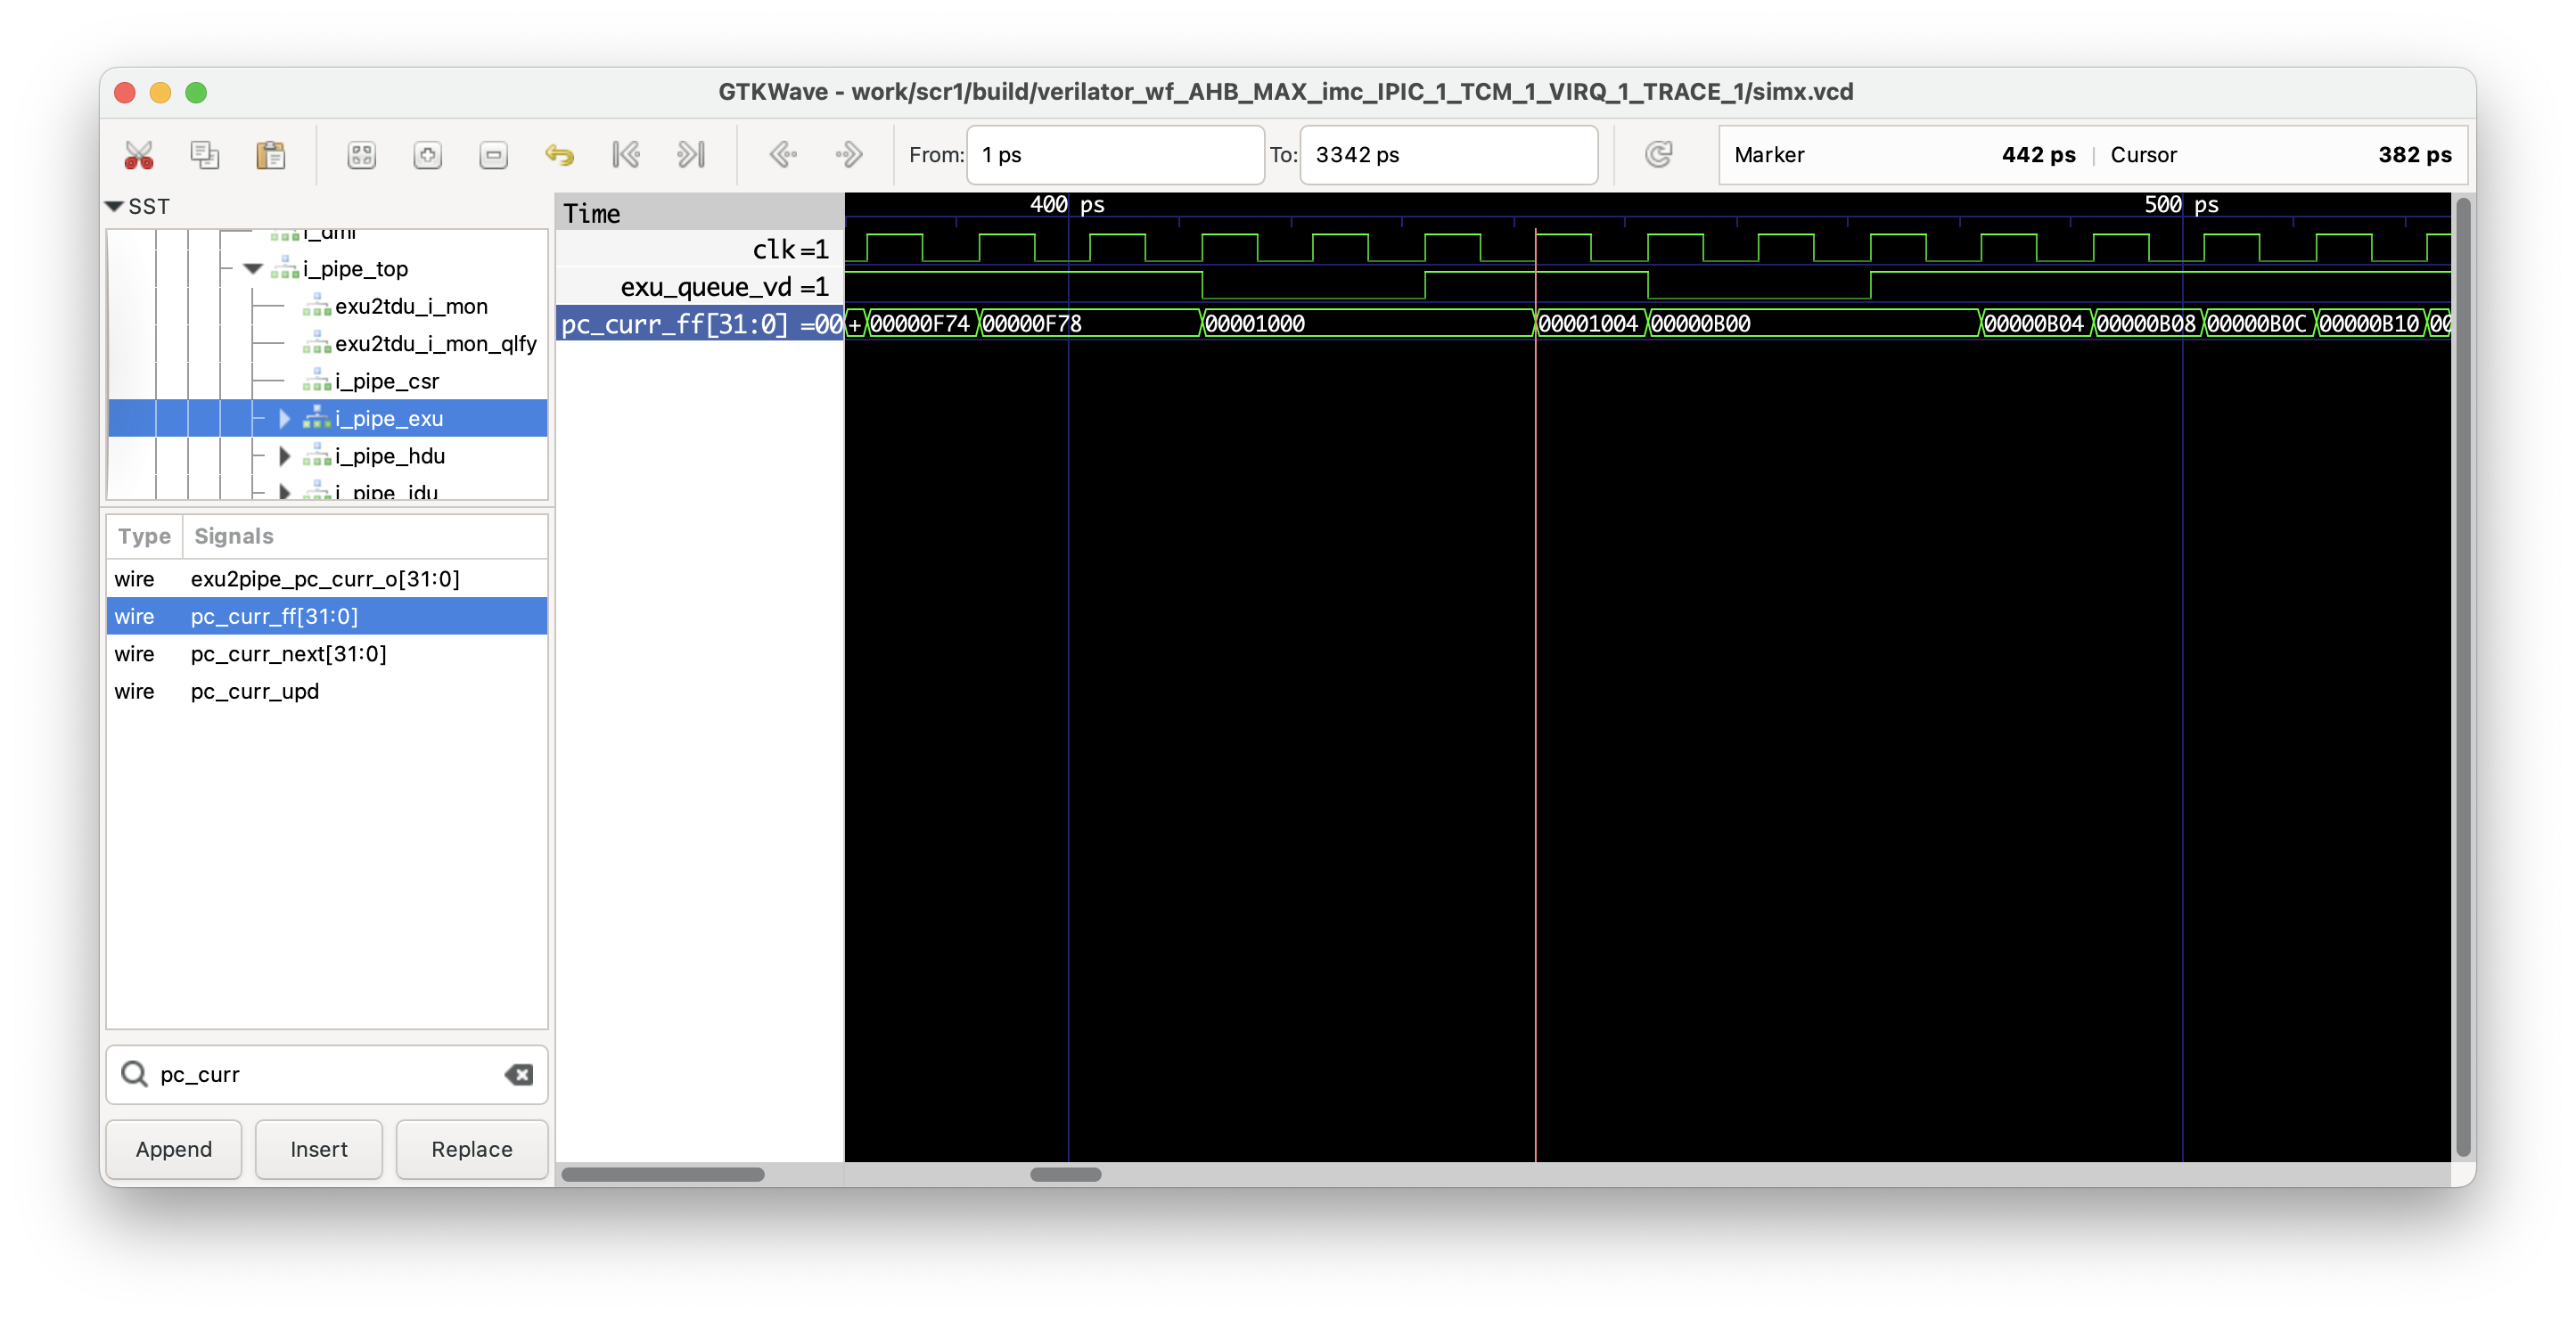
\includegraphics[width=\linewidth,trim={311bp 545bp 70bp 108bp},clip]{diagram.png}
\caption{Переход от недопустимой инструкции по адресу 0x1004
к общему обработчику по адресу 0xB00. Снимок GTKWave.}
\label{fig:illegal-trap}
\end{figure}

Последовательность значений PC на рисунке включает \texttt{0x1000},
\texttt{0x1004}, затем \texttt{0xB00}, \texttt{0xB04}, \texttt{0xB08}
и последующие адреса обработчика. Адрес \texttt{0x1004} соответствует
нулевому машинному слову в точке \texttt{bad2}; переход к \texttt{0xB00}
согласуется с установленным Trap Vector. Причина исключения подтверждается
отдельной трассой CSR: \texttt{mcause=2}, \texttt{mepc=0x1004}.
Признак \texttt{exu\_queue\_vd} показывает наличие действительной команды,
а не факт её завершения; значения PC при нулевом признаке не следует
трактовать как исполнение инструкции.
На этом снимке нет сигналов записи в порт \texttt{0xF0000000}, поэтому
вывод строки подтверждается журналом симуляции, приведённым выше.

\subsection{Вывод сообщения через порт симулятора}
На снимке ниже шина \texttt{dmem\_hwdata} отображена в ASCII-представлении:
последовательно читаются символы \texttt{incorrect instruction}.

\begin{figure}[htbp]
\centering
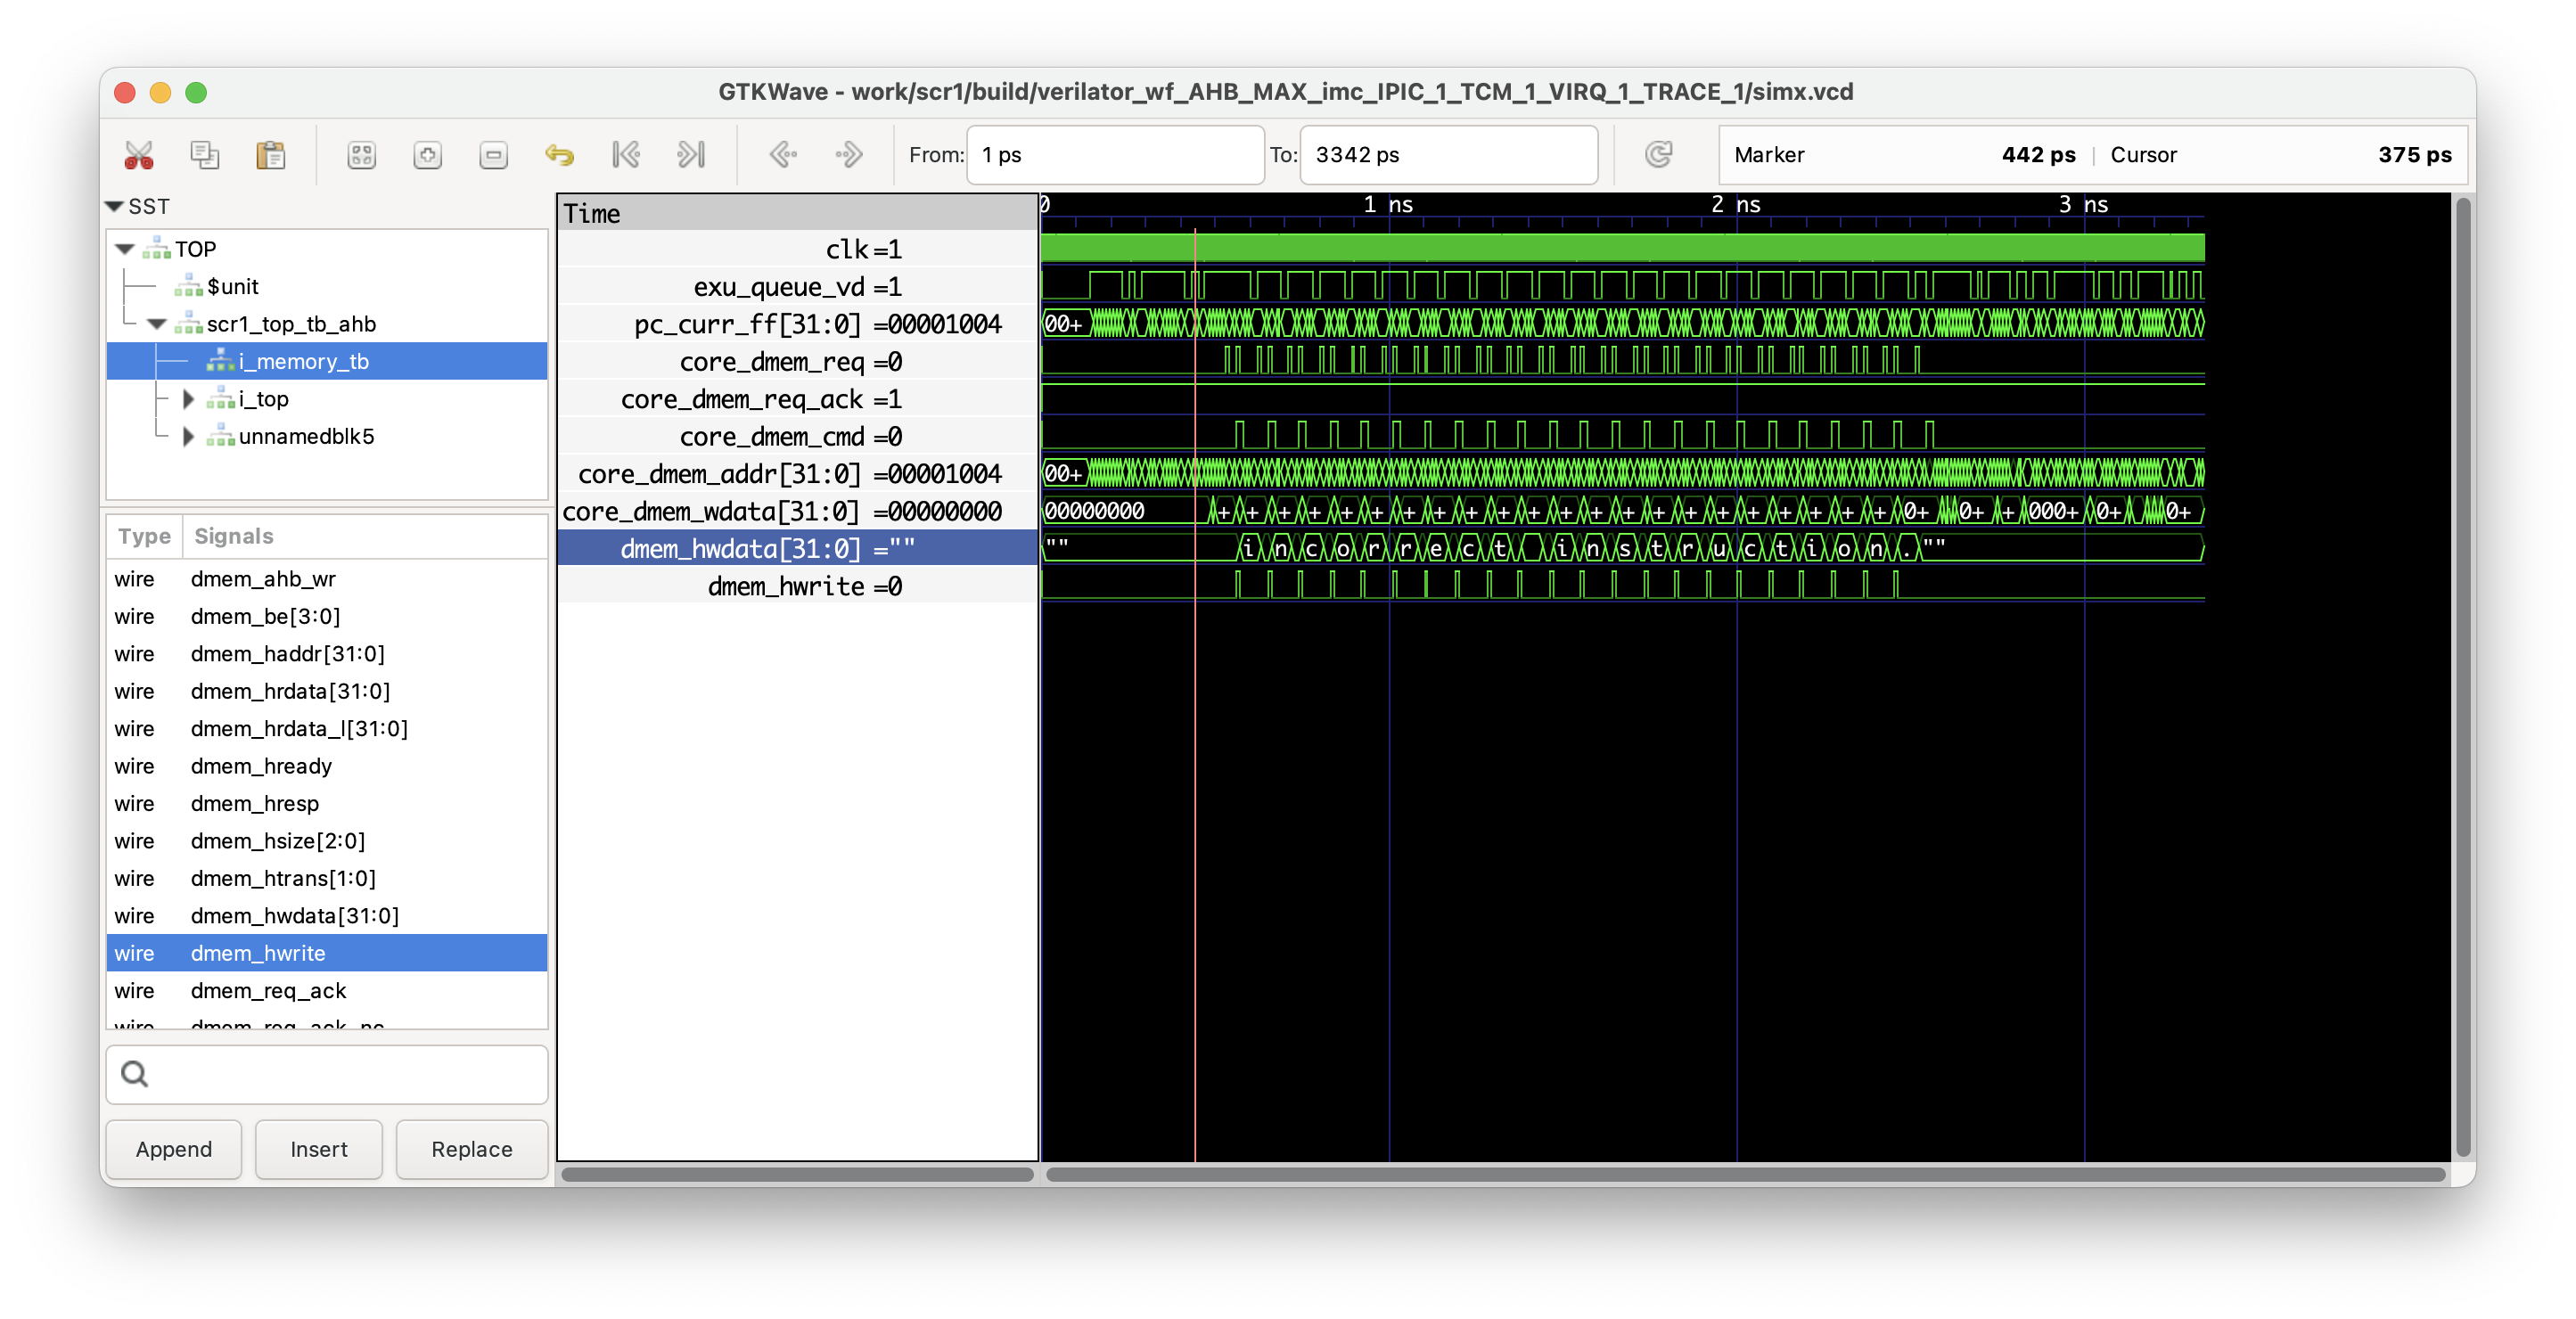
\includegraphics[width=\linewidth,trim={311bp 400bp 195bp 108bp},clip]{diagram-3.png}
\caption{Посимвольный вывод сообщения обработчика.}
\end{figure}

Обработчик читает байты строки и выполняет \texttt{sb} по адресу
\texttt{0xF0000000}. Начало сообщения кодируется байтами
\texttt{69 6E 63 6F 72 72 65 63 74 20} --- \texttt{incorrect} и пробел.
На стороне ядра запрос принимается на фронте \texttt{clk}, когда
\texttt{core\_dmem\_req=1} и \texttt{core\_dmem\_req\_ack=1}.
\texttt{core\_dmem\_cmd} различает чтение символа и запись в порт.

Сигналы \texttt{dmem\_hwrite} и \texttt{dmem\_hwdata} относятся к AHB.
Адресная фаза и фаза данных разделены, поэтому их нельзя автоматически
сопоставлять с текущим запросом ядра в тот же момент.
В данном масштабе адресная шина слишком плотная для чтения каждого адреса;
адрес порта подтверждается листингом, а снимок показывает передаваемую строку.
Значение шины вне действительной передачи не означает новую запись.

\section{Проверка выполнения пунктов задания}
\begin{longtable}{p{0.07\linewidth}p{0.39\linewidth}p{0.45\linewidth}}
\toprule
Пункт & Требование & Выполнение и подтверждение \\
\midrule
\endhead
1 & Личная копия через GitHub Fork &
Настроен личный SSH remote \texttt{origin}; исходный проект сохранён
как \texttt{upstream}. Сам факт создания GitHub Fork локальная
настройка remote не подтверждает. \\
2 & Ветка и исходная проверка &
Ветка \texttt{lab\_scr1\_sim}; сохранён исходный прогон 56/56 ISA.
Для остальных наборов исходного результата нет. \\
3 & Единственный тест варианта &
В \texttt{rv32\_tests.inc} оставлен \texttt{illegal.S};
одиночный исходный и итоговый прогоны успешны. \\
4 & Изменение \texttt{trap\_vector} &
Проверка причины 2, вывод \texttt{incorrect instruction},
сохранение передачи управления обработчику теста. \\
5 & Аппаратные векторы &
Reset Vector \texttt{0xF00}, Trap Vector \texttt{0xB00}. \\
6 & Компоновка и старт &
Секции \texttt{.text.trap}/\texttt{.text.reset}, фиксированные адреса
в \texttt{link.ld}; адреса проверены по dump. \\
7 & Артефакты в \texttt{results/} &
Итог теста, dump, MPRF-выборка и CSR-выборка сохранены.
Дополнительно сохранён исходный общий лог. \\
8 & \texttt{lab\_scr1\_sim/README.md} &
Создан файл с описанием и ссылками на подробные PDF и LaTeX
в \texttt{report/}. \\
9 & Коммит всех изменений &
Изменения реализации сохранены в рабочей ветке.
Новые отчёт и артефакты на момент проверки ещё не включены в коммит. \\
\bottomrule
\end{longtable}

Для окончательной сдачи требуется подтвердить статус Fork на GitHub,
согласовать с преподавателем объём исходной проверки либо выполнить
недостающие наборы и сохранить обновлённые материалы коммитом.
Последующий прогон уже изменённого проекта нельзя выдавать за исходный
прогон до изменений.

\section{Вывод}
Обработка Illegal instruction дополнена выводом заданной строки с сохранением
логики проверочного теста. Аппаратные Reset Vector и Trap Vector согласованы
с размещением секций программы: \texttt{\_start=0xF00},
\texttt{trap\_vector=0xB00}. По дизассемблированию и снимкам CSR подтверждены
правильный вход в обработчик, возврат после ожидаемого исключения и завершение
через \texttt{ecall}. Финальная симуляция единственного теста завершилась PASS.

\end{document}
